\section{Architecture}
\label{sect:architecture}

\subsection{Introduction}
A principle aim of this project was to design a component architecture for building scheduler implementations along with a simulation framework in which to test and measure the performance of these schedulers. As a preliminary step, prior to the start of this project, a simple despatch scheduler \cite{fraser04scheduling} was built for the LT to allow robotic science operations to start in 2004. The work on this scheduler and subsequent study of its operation provided insight into the range of components that would be necessary to design an architecture.

Some of the objectives in the design of the architecture are:-
\begin{itemize}
\item Hide the underlying database implementation from the scheduler.
\item Provide summarized version of the database content as scheduler does not require such detail.
\item Provide a range of standard, extendable tool interfaces.
\item Hide the scheduler implementation from executor.
\item Ability to make predictions about future conditions.
\item Time synchronization between scheduler and simulation framework.
\end{itemize}

It was a principle requirement that all components should be easily interchangable to suit the experiment. Most importantly, it should be feasible to plug an operational scheduler into a simulation environment with very little effort and with {\bf no} modification to the scheduler itself, it should in effect be unaware of whether it is scheduling real observations or not. The design would promote the use of Object Oriented interfaces to facilitate plugability.

In the forthcoming descriptions the following symbols are used:-

\begin{itemize}
\item $g$ A composite group (the group currently under consideration).
\notation{name={$g$},description={A composite group (the group currently under consideration)},sort={g}}
\item $t$ The current (real or simulation) time.
\notation{name={$t$},description={The current (real or simulation) time},sort={t}}
\item $a$ The set of account synopses apertaining to the current group.
\notation{name={$a$},description={The set of account synopses apertaining to the current group},sort={a}}
\item $h$ Synopsis of the execution history of the current group.
\notation{name={$h$},description={Synopsis of the execution history of the current group},sort={h}}
\item $e$ The current (at time t) environmental conditions.
\notation{name={$e(t)$},description={The current (at time t) environmental conditions},sort={e}}
\end{itemize}

\begin{landscape}
   \begin{figure}[htp]
   \begin{center}
   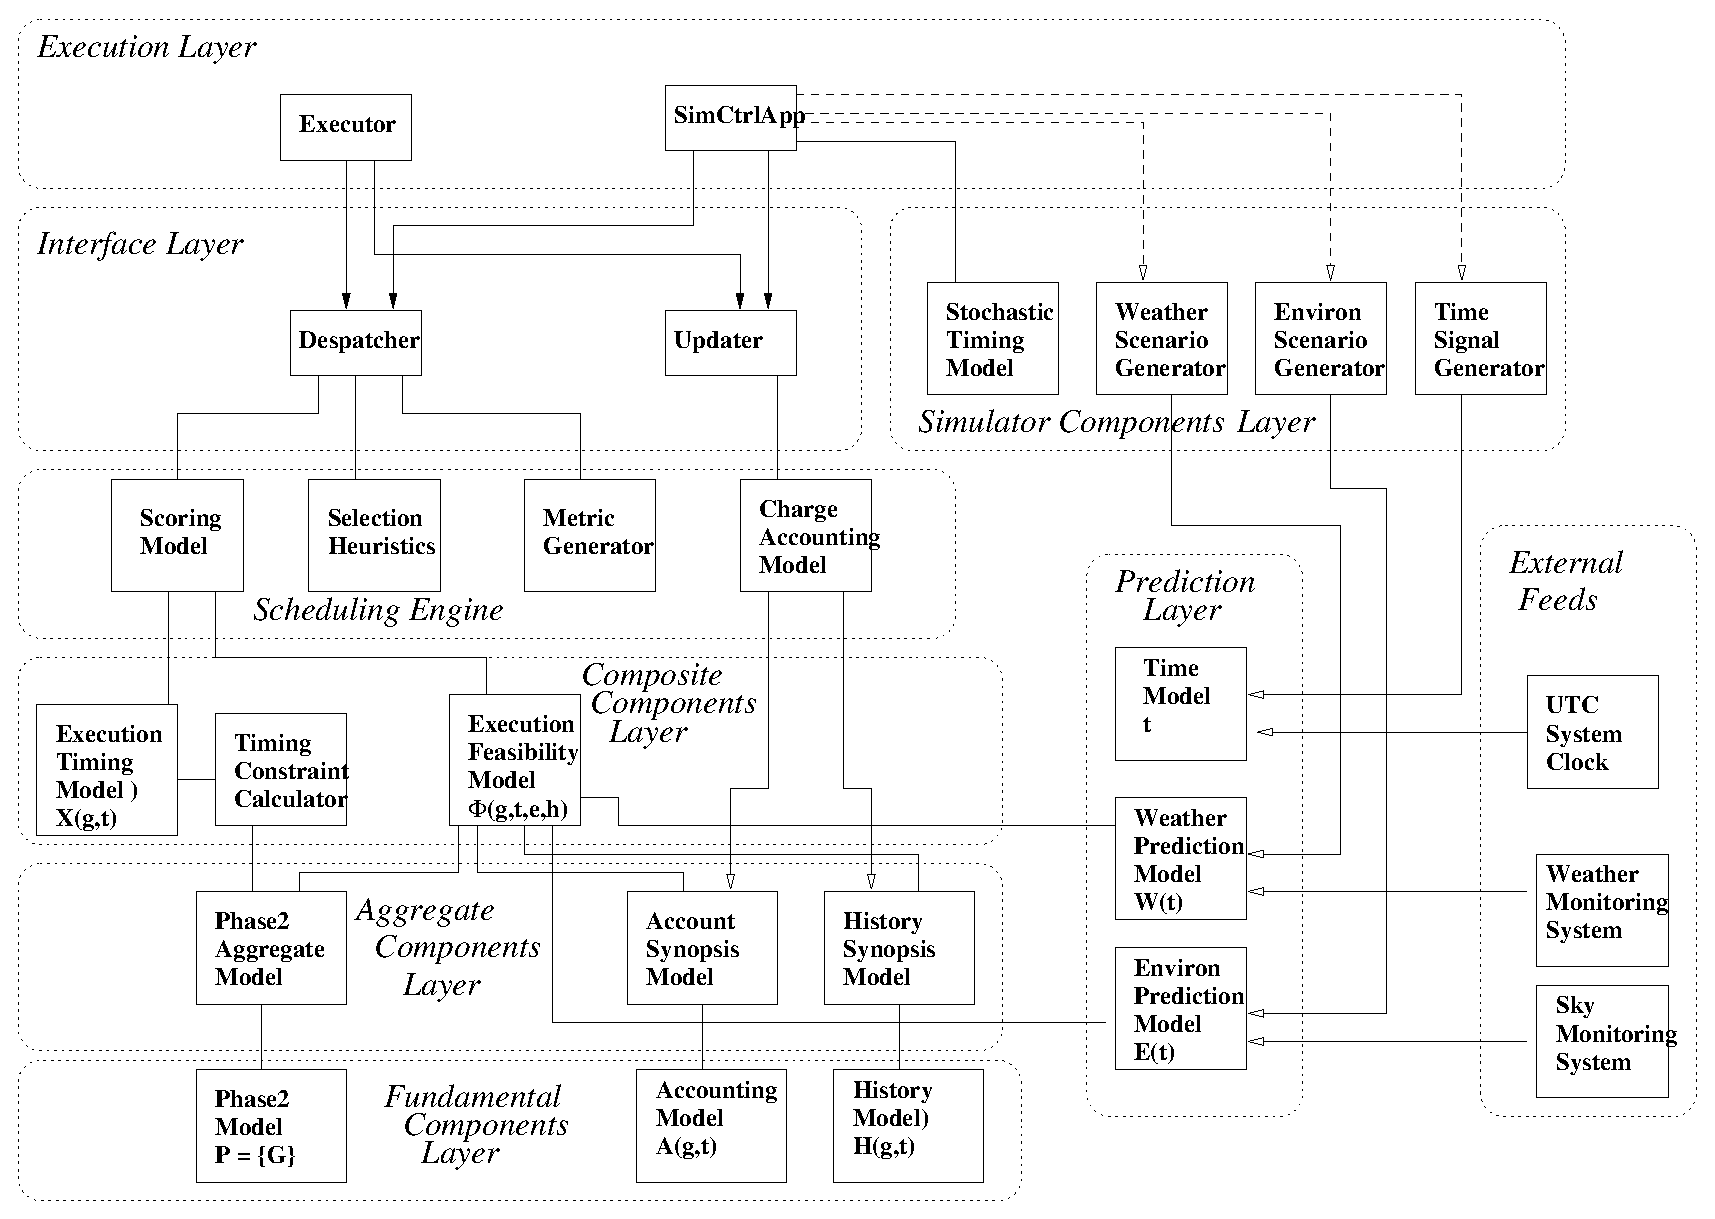
\includegraphics[height=14cm]{figures/sca.eps}
   \end{center}
   \label{fig:simframewrk} 
   \caption[Scheduler Component Architecture.] 
   {The Scheduler Component Architecture (SCA\glossary{name={SCA},description={Scheduler Component Architecture}}). This is split into a number of layers...described in the text.}
   \end{figure} 
\end{landscape}

%\glossary{name={},description={}}
\subsection{Fundamental Components Layer (FCL)}
\glossary{name={FCL},description={Fundamental Components Layer - part of the SCA, contains models for accessing the ODB}}
This layer contains models which provide access to the Phase II, Accounting and Group Execution history stored in the ODB. These models are used by the higher layers of the scheduling architecture and by the external Phase 2 User Interface services to query and update the database.

\subsubsection{Phase2 model} 
This is the information entered by the observers or on their behalf by automated agents which describes the content and constraints of the observing programs - i.e what to do and when. The information can be broken into the following categories:-

\begin{itemize}
\item Observation specifications contain details of the sequence of operations required to perform the observations; target selection, acquisition and tracking information, instrument selection, calibration and configuration, type, number and length of exposures, mosaicing offset patterns.
\item Timing constraints which determine when, how frequently and how many times to perform groups of observations.
\item Observing constraints impose limitations on the conditions under which observations may be taken.
\end{itemize}

\subsubsection{History model}
The history model (H) represents the record of execution histories of groups from the Phase 2 model. For flexibly scheduled single execution groups this is just the date/time it was executed. For repeating groups it represents the history of all of the times the group has been attempted (whether successfully or not) along with execution statistics. 

\subsubsection{Accounting model}
The allocation and use of resources by groups, proposals and TAGs is provided through the accounting model (A). When a proposal is created and on subsequent semesters if still active, the accounts for the proposal (and sponsoring TAG) are allocated new resources. When groups are executed the balance of relevant accounts is appropriately reduced. When observations are made but found to be sub-standard, the relevant account balance may be adjusted as \emph{payback}. All of these transactions are recorded in the ODB via the accounting model. The model also allows the scheduler or User Interface to trace the history of transactions via an audit trail.

\subsection{Aggregate Components Layer (ACL)}
\glossary{name={ACL},description={Aggregate Components Layer - part of the SCA, contains summaries of base models}}
The scheduling engine does not use the FCL models directly. Partly because much of the information contained in those models is more detailed or fine-grained than it requires to make scheduling decisions and more importantly for the sake of efficiency, the ACL provides synposes of the FCL models. When running in a simulation environment, rather than generating the basic FCL models, the simulation controller usually generates the models in this layer directly.

\subsubsection{Phase 2 Composite Model}
The Phase 2 Composite Model (P2C) provides a \emph{group-centric} view of the Phase 2 ODB content. In addition to the sequencing, timing and observing constraints the \emph{composite} groups provided by this model contain details of the owning proposal, TAG, program and PI. 

\subsubsection{Account Synopsis Model}
This model provides a single point \emph{account synopsis} for each proposal containing details of all of the proposal's accounts for each valid semester. The synopses contain balance information but do not provide a detailed audit trail facility.

\subsubsection{History Synopsis Model}
Details of the latest successful execution and number of executions upto a given date are provided by this model.

\subsection{Computational Tools Layer (CTL)}
\glossary{name={CTL},description={Compuational Tools Layer - part of SCA, provides processing capabilities}} 
The CTL provides models and tools for processing information derived from the ACL. These are the scheduler's models of the function of the executor, whether RCS or simulation controller. Computing models such as the \emph{execution timing model} $X(g,t)$ which provides details of the time required to execute groups by modelling the function of the execution system and the \emph{feasibility model} $\Phi(g,t,e,h)$ which determines the potential observability of groups under given environmental conditions. The astrometric tools can also be considered part of this layer.

\subsubsection{Execution timing model}
\label{sect:sub_xtm}
Provides details of resource consumption of groups of observations, answering questions like:- \emph{how long will it take to complete group x ?}. Information relating to the telescope, instruments and robotic system are combined to make these estimates based on the primitive operations described by the group's observation sequence. Some of these components can be characterized well, others provide a source of uncertainty. In the standard model used in the deployed system, Table.~ \ref{tab:exectime_factors} describes which events in an observing sequence are used to make the estimation:-


% CONFIG VAR TABLE
\begin{table}[htbp]
\begin{center}
\begin{tabular}{lp{20em}}
\toprule
\multicolumn{2}{c}{Factors involved in calculation of execution time.} \\
\midrule
Time factor & When required \\
\midrule
Slew rate in each axis & Target changes, position offsets, rotator mode or angle changes, rotator cardinal pointing solution changes.\\
Instrument filter defocus time & Instrument or filter changes. \\
Fold mirror move/deploy & Instrument changes, some calibrations. \\
Instrument configuration & Movement of filter wheel, grating or other internal mechanism. \\
Instrument calibration & Lamp-flats, darks, biasing, arcs. \\
Fine-tuning & Acquisition by an instrument onto spectrograph slit \\
Autoguider acquisition & When switching autoguider on. \\
Aperture offsets & Instrument changes. \\
Readout time & Exposures, may depend on binning and windowing \\
Data write-to-disc time  & Exposures, may depend on binning and windowing. \\
\bottomrule
\end{tabular}
\end{center}
\caption[Factors involved in calculation of execution time for groups.]
{Factors involved in calculation of execution time for groups.}
\label{tab:exectime_factors}
\end{table}


\subsubsection{Execution feasibility model}
\notation{name={$\Phi(g,t,e,a,h)$},description={Feasibility model, determines whether a particular group is feasible subject to its constraints and under specified conditions},sort={F}}
Generally denoted by the symbol $\Phi(g,t,e,h,a)$ this model is used to determine whether a particular group is feasible subject to its constraints and under specified conditions. A number of factors are taken into account in the operationally deployed system:-

\begin{itemize}
    \item \emph{Seeing} - The actual seeing, corrected for airmass and wavelength to a standard datum (zenith, r-band) is compared to that specified in any seeing constraint.
% A group can be observed in better conditions but not worse. Seeing is determined from real-time reductions of science and photometric standard frames as they are obtained. Corrections are automatically applied for zenith distance and filter wavelength. The seeing value you set in the observing constraint is compared against the scheduler's prediction for the what image quality will be acheived in the r-band taking into account the current airmass of your target. For example, if you request AVERAGE seeing conditions, the scheduler might attempt the observation at any airmass if the current seeing is very good, but if the seeing is only average it might reject your target when low on the horizon because it predicts the conditions will be poor there. Scheduling is always performed on an assumption of r-band so you might expect for example, u-band images to show FWHM larger than the criterion set in the observing constraint.
    \item \emph{Lunar elevation} - The moon must be set for groups which specify a Lunar Elevation constraint.
    \item \emph{Lunar distance} - All targets in a group's sequence must be a minimum distance on the sky from the moon.
    \item \emph{Hour-angle} - All targets in the group must fall within specified HA limits in order to be observed.
    \item \emph{Solar elevation} - The sun's elevation is compared to the requested level of twilight or astronomical darkness.
    \item \emph{Airmass} - All targets in a group must remain above the specified airmass for the duration of the group's execution.
    \item \emph{Extinction} - Extinction is determined early in the night. If the group requires Photometric conditions and the current conditions are poorer it will not be selected.


    \item \emph{Horizon} - All targets in a group must be visible above the dome horizon, typically 20 - 25 degrees depending on any engineering settings, for the full duration of the group.
    \item \emph{Zenith} - Targets must not cross the zenith avoidance zone (ZAZ) during an observation. This is a very narrow zone around the zenith imposed due to speed limitation of the cassegrain rotator tracking.
    \item \emph{Time limit} - The RCS may impose time limits by which groups must have completed such as for performing important calibration observations. Groups will not be selected if they are expected to overrun into such periods.
    \item \emph{Daytime} - Groups will not be selected if they are expected to overrun into daytime.
    \item \emph{Allocation} - A group cannot be selected if the containing proposal's total time allocation will become overdrawn.
    \item \emph{Activation} - If a proposal is outside of its activation period no groups can be selected from it.
    \item \emph{Axis Limit} - No target in a group may cross outside any temporary axis range which may be imposed for engineering reasons from time to time.
    \item \emph{Instrument} - If any observation in a group specifies an unavailable instrument, or a configuration which is not currently available for an instrument, or the instrument is impaired, the group cannot be selected.
    \item \emph{Fixed group} - If a fixed group is due before a candidate group can be expected to complete (with a short buffer time to allow slewing onto target) then that group cannot be selected.
    \item \emph{Autoguider} - It is possible to specify mandatory, optional or no autoguider use. If the autoguider is reported as unavailable or impaired, groups which require mandatory use of this will not be selected.

\end{itemize}


\subsubsection{Astrometry}
The astrometry library provides tools to work out where various types of target (stars, planets, NEOs and the sun and moon) are on the sky. Additionally it provides tools to determine rising, setting and transit times of objects and various transformations between coordinate systems.

\subsection{Prediction Components Layer (PCL)}
\glossary{name={PCL},description={Prediction Components Layer - part of SCA, provides predictive models}}
 Contains models for predicting sky and weather conditions and a \emph{time model} which provides a synchronizing time signal. %In an operational situation this is simply the system clock. In a simulated environment it is provided by the simulation controller's time signal generator component.
 In an operational context these models are fed from external sources such as the weather monitoring system (WMS), the sky conditions model and the instrument and telescope monitoring systems. In a simulation environment these components can be setup to perform predictions of whatever degree of accuracy is required by tying their predictions to scenarios generated by the components in the SFL (Sect.~\ref{sec:sub_sfcl}).

\subsubsection{Environmental Prediction Model}
During both operational and simulated execution scheduler need to have available a prediction of the sky conditions. In the case of a despatch scheduler the requirement is simply for the current conditions. In an operational context this information is generated by reduction of the images from the main imaging camera via a real-time pipeline algorithm \cite{lt11pipelines}. These are fed into the model and an exponential averaging applied so that recent reductions have higher weight than older reductions. In the case of a look-ahead scheduler the requirement is to determine both the current conditions and how far into the future these conditions will remain stable in order to deduce a suitable sequence horizon. In a simulation context this information can be provided by an Environmental Scenario Generator (Sect.~\ref{sect:sub_esg}). The prediction can be made to be as accurate or innacurate as the experiment requires. In an operational context, prediction of environmental conditions is somewhat more difficult, a more detailed discussion on this subject is to be found in Sect.~\ref{sect:sub_atmoseeing}. In the experiments a number of Environmental Prediction Models are used. Fixed environment models $E_{FP}$, $E_{FA}$, $E_{FX}$ \notation{name={$E_{FP}$},description={Fixed environment model with poor ($>1.3$'') seeing},sort={E}} \notation{name={$E_{FA}$},description={Fixed environment model with average ($0.8''< s <1.3''$) seeing},sort={E}} \notation{name={$E_{FX}$},description={Fixed environment model with excellent ($<0.8$'') seeing},sort={E}}  etc are used in the simulations in Sect.~\ref{sect:exp_scoring}. A more advanced model is described in Sect.~\ref{sect:exp_stability} in the context of measuring the effect of environmental stability on scheduling. 


\subsubsection{Weather Prediction Model and Disruptor Model}
Disruptions are any events which can stop the execution of the observing program. These include:- bad weather, mechanical, electrical and hydraulic faults and software problems leading to node reboots. If the scheduler knew in advance when these events were going to occur it could take them into account in its decision making process. With the exception of weather for which there is at least some limited potential for future prediction, the other types of event are by their nature unpredictable. This is not to say however that some account cannot be taken of these. We can at least obtain long-term averages of the rates and duration of these types of event and feed this information into the scheduler. In the operational context, a despatcher requires only the current weather, though ideally an estimate of the likelihood of the weather remaining good for the length of a group under consideration would be useful. Weather information is supplied by the telescope's Weather Monitoring System (WMS) via various filtering mechanisms supplied by the RCS. In a simulation context weather and other disruptor information is supplied by a Weather or Disruptor Scenario Generator (Sect.~\ref{sect:sub_wsg}). The weather or disruptor prediction can be made to any desired degree of accuracy required by the experiment. In Sect.~\ref{sect:exp_disruption} the effects of such disruptions are studied.


\subsubsection{Instrument Synopsis Model (ISM)}
\glossary{name={ISM},description={Instrument Synopsis Model}}
This model provides information on the state of each of the instruments attached to the telescope and thus available for use in the execution of groups. Where a given instrument is either \emph{offline} or \emph{impaired}, a group using the instrument cannot be selected for execution. By coupling an ISM with a scenario generated by an ISG (Sect.~\ref{sect:sub_isg}) any evolving instrument availability scenario can be handled. Because this model is a synoptic model rather than a predictive model it basically answers the question \emph{Is instrument x available at current time t ?} rather than the question \emph{Will instrument x be available at future time t ?}. Some care has to be taken particularly in the implementation of look-ahead schedulers to ensure the scheduler only sees the instrument's known state at the simulation time rather than its true state at a future time as would be known to the ISG.

\subsubsection{Telescope Synopsis Model (TSM)}
\glossary{name={TSM},description={Telescope Synopsis Model}}
Similar to the ISM, the TSM provides information about the telescope state. In particular the state of the autoguider system is of interest to the scheduler as groups for which use this instrument is mandatory cannot be scheduled if it is \emph{non-operational}. Similar considerations with respect to scenario generation and visibility of information which apply to the ISM also apply to the TSM. A TSM can be coupled to a TSG scenario (Sect.~\ref{sect:sub_ssg}).

\subsubsection{Time Model} 
This model simply supplies the current time to any components. In an operational context this is represented by the system clock. In a simulation context the time signal is coupled to the Time Signal Generator (Sect.~\ref{sect:sub_tsg}).


\subsection{Simulation Framework Components Layer (SFCL)}
\glossary{name={SFL},description={Simulation Framework Components Layer - part of the SCA, provides models used by simulators}}
\label{sec:sub_sfcl} Provides \emph{scenario generators} with which to build a simulation environment incoporating time-varying and random effects (weather and sky conditions). A \emph{stochastic timing model} simulates variable execution timing due to uncertainty in mechanical and software processes while a seperate signal generator provides a time signal to the simulation controller.

\subsubsection{Environmental Scenario Generator}
\label{sect:sub_esg}
This allows an environment (sky conditions) scenario to be represented. It can be taken from actual processed sky conditions data or generated using statistical or other means. From the scheduler's point of view, it is not usually bothered about the actual precise details of how the seeing value is changing from minute to minute, just the general classification of conditions into extinction as photometric/non-photometric and seeing into one of the 3 or 4 pre-defined bands.

\subsubsection{Weather Scenario Generator and Disruptor Scenario Generator}
\label{sect:sub_wsg}
This allows a weather scenario to be represented. It can be taken from actual processed weather data or generated from statistical measurments or other means. As with environmental scenario we only need to know if the weather is good or bad not the details though this level of detail may be needed for prediction modelling.

\subsubsection{Time Signal Generator (TSG)}
\label{sect:sub_tsg}
\glossary{name={TSG},description={Time Signal Generator - a SCA component which synchronizes the scheduler with its simulation controller}}
The Time Signal Generator (TSG) is vital to the operation of the simulation framework. It allows the simulation controller to synchronize with the executing scheduler and any real-time operations being performed. More details of this component are to be found in Sect.~\ref{sect::experiments}.

\subsubsection{Stochastic Timing Model}
Although the execution timing model ($X$) described in Sect.~\ref{sect:sub_xtm} allows the scheduler to estimate the duration of a group execution, the actual execution duration may vary for a number of reasons including:-

\begin{inparaenum}[(\itshape i\upshape)] \item A slew can take anything upto 180 secs, \item Fine-tuning acquisition onto a spectrograph fibre can take upto 60 secs, \item autoguider lock can take upto 60 secs, \item science fold movement between instrument ports can take upto 40 secs, \item imager configuration time depends on the start and end filter positions on the wheel and direction of travel, \item exposure readout times can vary to a small extent but where a large number of short exposures is performed this can be significant.\end{inparaenum}.
The Stochastic Timing Model allows this variation to be modelled in a simulation context. This is the size of the time-step for the simulated completion of a group. The distribution of times around the nominal value calculated by the execution timing model  depends on the specific model used. Fig.~\ref{fig:simf_exec_timing_dist} shows the results of 2 methods of implementing a stochastic timing model for a sequence containing 3 slews and 3 instrument configurations. The flat plot is the result of adding a random variation to the total calculated execution time from an implementation of the Execution Timing Model. The curved plot shows the results of modelling each of the variable processes then adding the results.

\begin{figure}[h]
\begin{center}
  \includegraphics[scale=0.5, angle=-90]{figures/simf_exec_plot.eps}
\caption[Distribution of execution times for stochastic execution model]
{Distribution of execution times for stochastic execution model. \emph{Mono} plot uses a single calculation to total up contribution of all events, \emph{multi} plot works out a seperate random effect for each contributing event. In most of the experiments the mono version was used for simplicity.}
 \label{fig:simf_exec_timing_dist}
\end{center}
\end{figure}

\subsubsection{Instrument Scenario Generator}
\label{sect:sub_isg}
Allows the time evolving state of the instruments to be modelled. In general this is just setup so that all instruments are always online and available. If there were an experimental requirement to disable one or more instruments for a period such a feature would be implemented here.

\subsubsection{Telescope Scenario Generator}
\label{sect:sub_ssg}
Allows the time-evolving state of the telescope systems to be modelled. The most important component being the autoguider status. When this is offline or impaired, any groups with mandatory autoguider use become infeasible.

\subsection{Scheduling Engine Component Layer (SECL)}
\glossary{name={SECL},description={Scheduling Engine Components Layer - part of the SCA}}
The components in this layer largely determine how a scheduler functions. Implementations of the heuristics and logic of the scheduler algorithms are specified here. In addition to basic scoring and selection mechanisms, other scheduler-specific algorithms would be included here. This layer is in effect what would be described as \emph{the scheduler}. 
%Provides \emph{selection heuristics} used to select single groups (or sequences of groups) for execution using the scoring/utility metrics provided by the \emph{scoring model} $S(g,t,e,a,h)$ which determines the gain from performing a specified group. The \emph{cost accounting model} calculates the chargeable cost of performing a group - the time which will be deducted from the proposal's allocation.

\subsubsection{Scoring Model}
\notation{name={$S(g,t,e,a,h)$},description={Score for a group $g$ at time $t$ under specified account balance, history and environment conditions},sort={S}}
\label{ss:scoring_model}
Calculation of the score ($S(g,t,e,a,h)$) for a group at a given time and with the specified execution history $h$, account synopsis $a$ under environmental conditions $e$ from a set of metrics is provided by an implementation of this model . A number of schedule quality metrics were defined in Sect.~\ref{sect:metrics}. The differential versions of these SQMs are frequently used as scoring metrics. typically for a $Q$ metric such as $Q_{x}$ the equivelant scoring metric is denoted $f_{OA} = \dot{Q_x}$ \notation{name={$f_x$},description={Scoring metric derived from $Q_x$},sort={f}}.

\begin{itemize}
 
\item \emph{Height metric} $f_h$ \notation{name={$f_{h}$},description={Scoring metric based on target elevation},sort={f}} simply measures the elevation of the group's target at the time of potential observation. Variations on this metric can inlcude taking the mean or peak elevation over the duration of the group. If a group has multiple targets various averages can be used such as taking mean elevation of each target at some point in the execution. More complex averages could take into account the actual times at which each target will be observed. 
 
\item \emph{Airmass metric} $f_{air}$ \notation{name={$f_{h}$},description={Scoring metric based on target airmass},sort={f}} is similar to $f_h$ except that the airmass is used rather than elevation thus taking into account the nonlinear nature of the relationship between sky-quality and elevation.

\item \emph{Transit metric} $f_{trans}$ \notation{name={$f_{trans}$},description={Scoring metric derived from $Q_{OH}$},sort={f}} is an attempt to take into account the unfair advantage provided by the two previous metrics $f_h$ and $f_{air}$. These force a bias towards targets whose declination is close to the latitude of the observatory. This metric measures the quality of observing at a given time by taking the current target elevation as a fraction of its \emph{best} elevation. This is generally taken as its transit elevation which can be calculated easily. For groups which do not transit during the feasibility window and in particular for groups with very short feasibility windows this may still be somewhat unfair as the transit elevation may not be remotely achievable in that window.

\item \emph{Optimal elevation} $f_{oh}$ and optimal airmass $f_{oa}$ metrics attempt to redress this problem by taking the ratio of current elevation to \emph{best possible} elevation (or airmass) in the group's feasibility window. \notation{name={$f_{oh}$},description={Scoring metric derived from $Q_{OH}$},sort={f}} \notation{name={$f_{oa}$},description={Scoring metric derived from $Q_{OA}$},sort={f}}

\item \emph{Slew metric} $f_{slew}$ \notation{name={$f_{slew}$},description={Scoring metric based on reducing slewing overheads},sort={f}} attempts to penalize groups for which a long axis slew (including rotator) from the current telescope position is required. This can prove very difficult to calculate as it requires the scheduler to predict the way the executor will choose rotation angles. The recently introduced cardinal pointing (CP\glossary{name={CP},description={Cardinal Pointing - a restricted operating regime for the rotator axis}}) regime on the LT, to handle the problem of coolant pipes in the wrap, makes this somewhat easier to determine.

\item \emph{Sky condition matching metric} $f_{see}$ (also $f_{phot}$ and $f_{sky}$) is designed to match a group's sky condition requirements to the actual (or predicted) conditions at the time of execution. This is intended to ensure that groups which do not require particularly good conditions do not take an excessive share of good conditions. \notation{name={$f_{see}$},description={Scoring metric based on matching requested and actual seeing},sort={f}} \notation{name={$f_{phot}$},description={Scoring metric based on matching requested and actual extinction},sort={f}}

\item \emph{Lunar condition matching metric} $f_{moon}$ is similar to the above but attempts to prevent groups which can use \emph{bright} time from taking an excessive share of \emph{dark} time.\notation{name={$f_{moon}$},description={Scoring metric based on matching requested and actual sky brightness},sort={f}}

\item\emph{Priority metric} $f_p$ is designed to ensure that groups of higher scientific priority get a better share of time. \notation{name={$f_{p}$},description={Scoring metric derived from $Q_{PX}$},sort={f}}

\item \emph{Resource allocation metric} $f_{a}$ measures the use of various resources by a group or its containing proposal. This is typically the use of time from the proposal's total semester allowance. It can be used either to help distribute time fairly between proposals or to force completion of proposals which have already been started.

\item \emph{Demand metric} $f_{td}$ uses the group's demand for time as an indication of the urgency of performing the group (Eq.~\ref{eq:demand}). The idea behind this is to select the groups which have the most critical requirment for a given time period. \notation{name={$f_{td}$},description={Scoring metric derived from $Q_{TD}$},sort={f}}

\item \emph{Urgency metric} $f_{rn}$ is similar to the demand metric but measures the number of additional chances (in terms of alternative nights on which the group \emph{could} be observed if not tonight.\notation{name={$f_{rn}$},description={Scoring metric derived from $Q_{RN}$},sort={f}}

\item \emph{Yield tracking metric} $f_{yt}$ tracks the deficit in data product yield. This is basically the difference between the amount of data that might have been expected if all of a group's observations had been performed at each occasion when they could have been. In order to calculate this metric, both past and future yield estimates and yield to-date are required for each active group. This is an expensive calculation as the set of feasible and available windows have to be calculated over possibly an extended period (e.g. a whole semester).\notation{name={$f_{yt}$},description={Scoring metric derived from $Q_{YT}$},sort={f}}

\end{itemize}

\subsubsection{Selection Model}
Given a set of weighted scores or a set of raw metrics, the Selection Model ($\zeta$) chooses which group or sequence of groups to execute next or over the next horizon.  In the experiments (Sect.~\ref{sect:exp_complexity} and others) several selection models are used. In the \emph{Best} selection model, the highest scoring group is always selected. In the various \emph{biased} selection models a degree of noise is added so that sometimes the highest scoring group is not selected. In certain experiments, a self-explanatory \emph{random} selection model is empoyed.\notation{name={$\zeta$},description={Scheduler candidate selection model},sort={z}}

\subsubsection{Metric Generator}
This component works out the set of metrics appropriate to a group at a given time under specified conditions. The set of metrics can then be used to calculate a score (ScoringModel) or inspected to apply some other type of criterion to determine a winner. An example is to pick the group for which some metric $m1$ is highest, then if tied select the group for which $m2$ is highest.

\subsubsection{Charge Accounting Model}
When observers prepare their proposals to go before the TAG for time and resource allocation the cost or charging model ($C$) is  used to calculate the amount of time the groups \emph{should} take to execute. In the operational context, standard figures for slewing, acquisition, readout and instrument configuration are published on the telescope website for observers to calculate their resource requirements. These values are used to calculate the nominal cost of performing a group. In reality a group may take more or less time than this but this is the resource usage which is charged to the relevant account. This model is exposed through the Phase 2 User Interface to allow observers to determine these costs in advance.


\subsection{Interface Components Layer (ICL)} 
\glossary{name={ICL},description={Interface Components Layer - part of the SCA, contains interfaces used by the executive components}}
The executive, whether it be an actual robotic control system or a simulation control application, communicates with the scheduler via the components in this layer. The \emph{despatcher} is the executive's entry point for obtaining a schedule and the \emph{updater} allows the executor to supply observation completion statistics back to the fundamental component models. (e.g. to let the history model know that a group was successfully executed).

\subsubsection{Despatcher}
The despatcher interface is where the execution system makes requests for new groups of observations to perform. In the case of a despatch scheduler (BDS) this is the signal to make a scheduling sweep. In the case of an operational Look-ahead scheduler the sequence for the current horizon should already have been generated in advance, the despatcher then just pulls the next group off the pre-compiled sequence. In the case of QLAS (Sect.~\ref{ss:sched_impl}) the signal to generate a sequence is triggered by the first call to the despatcher. Thereafter it returns the next unexecuted group from the sequence till the horizon is exceeded or the list runs out. It then generates a new sequence on the following call. This would be inefficient for an operational system where the executor might have to wait a significant period at the end of each horizon but is quite acceptable in a simulation environment.

\subsubsection{Updater}
When a group has completed, whether successful or not, the executor must pass information back down to the database to record the state of this execution and to allow the sponsoring proposal and TAG accounts to be debited. The Updater provides this interface. It may directly modify the ODB via FCL components or may update the cached models in the ACL which then propagate these changes via the FCL to the ODB. When a group fails for some reason, the history model receives information detailing the cause of the error which can be useful for users and operations staff in diagnosing problems.

\subsection{Executive Components Layer (ECL)} 
\glossary{name={ECL},description={Executive Components Layer - part of the SCA, contains the external applications which invoke the scheduler}}
Represents the external application which requires the services of the scheduler. This will either be the telescope's Robotic Control System, a simulation control application or a user tool.
\subsubsection{Executor}
This component represents the system which performs the observations. In an operational system, this is the robotic control system of the telescope. Its general cycle of operation involves repeating the following sequence:-

\begin{enumerate}
\item Request next group from \emph{Despatcher}. 
\item Decompose observing sequence and send commands to telescope and instruments.
\item Send completion information to \emph{Updater}.
\end{enumerate}

\subsubsection{Simulation Controller}
For each simulation experiment a controller application must be designed. It is responsible for setting up any generated models and scenarios and for performing the observations. Additional details of simulation operations are provided in Sect.~\ref{ss:sim_ops}.
